% !TeX root = ../tesis.tex

\chapter{Eritrocitos y sus patologías}
En este capítulo se estudia la morfología, la composición y las principales alteraciones patológicas de los eritrocitos, y se derivan las funciones dieléctricas correspondientes a distintas concentraciones de hemoglobina a partir de datos reportados en la literatura. En la primera parte se describe la composición y las características generales de la sangre, para posteriormente centrarse en los eritrocitos, analizando su forma, su variabilidad morfológica y los cambios en la concentración de hemoglobina corpuscular media (CHCM) asociados a diversas enfermedades. En la segunda parte se introduce un modelo geométrico del eritrocito basado en óvalos de Cassini, el cual permite representar de manera realista su forma bicóncava \cite{ereminaDifferentShapeModels2006a}. A continuación, se presentan y analizan las propiedades ópticas de los eritrocitos y del plasma en el rango ultravioleta–visible, con énfasis en la dependencia de la función dieléctrica con la CHCM. Se discuten los datos experimentales disponibles para las partes real e imaginaria del índice de refracción de la hemoglobina a distintas concentraciones y su formulación en términos del incremento refractivo específico \cite{friebelModelFunctionCalculate2006}. Con el fin de obtener representaciones analíticas de los datos experimentales, la parte imaginaria de la función dieléctrica se ajusta mediante un modelo de osciladores de Lorentz y la parte real se reconstruye empleando las relaciones SSKK. Finalmente, se interpretan las principales características espectrales de la hemoglobina, en particular la banda de Soret en el ultravioleta y visible y las bandas Q en el visible, que dominan la respuesta óptica de los eritrocitos \cite{dayerBandAssignmentHemoglobin2010}.

\section{Morfología y enfermedades}
\label{section:results}


La sangre humana está compuesta principalmente por eritrocitos —también conocidos como glóbulos rojos (RBCs, por sus siglas en inglés)—, leucocitos, plaquetas y plasma sanguíneo~\cite{mescherJunqueirasBasicHistology2024}. El plasma constituye el medio continuo en el que se encuentran suspendidos estos elementos y está formado por agua, electrolitos, proteínas plasmáticas, carbohidratos, lípidos y diversas vesículas extracelulares \cite{mescherJunqueirasBasicHistology2024}. Si bien el plasma presenta absorción y esparcimiento óptico, originados principalmente por proteínas como la albúmina y el fibrinógeno, así como por las plaquetas, su contribución a la respuesta óptica global de la sangre en el rango espectral de 250 a 1100 nm es despreciable \cite{meinkeOpticalPropertiesPlatelets2007a}. No obstante, bajo ciertas condiciones patológicas, dicha absorción puede incrementarse \cite{bosschaartLiteratureReviewNovel2014a}. En contraste, dentro de ese mismo rango espectral, la respuesta electromagnética de la sangre está dominada por los eritrocitos, cuya contribución puede superar hasta por tres órdenes de magnitud la de los demás componentes \cite{bosschaartLiteratureReviewNovel2014a}. Esta diferencia se debe al contraste entre su índice de refracción y el del plasma \cite{bosschaartLiteratureReviewNovel2014a}. Por ello, para describir la interacción luz–sangre, en este trabajo se consideran únicamente a los eritrocitos y al plasma: el primero actúa como la partícula esparcidora  y el segundo como el medio circundante.

 
 Los eritrocitos son células terminalmente diferenciadas\footnote{Una célula terminalmente diferenciada se define como aquella que, al adquirir funciones especializadas, pierde su capacidad de proliferar de manera irreversible. Por ejemplo, los eritrocitos y queratinocitos de los mamíferos,
	sufren una detención irreversible de su crecimiento al perder su núcleo durante la diferenciación terminal \cite{saccoCellCycleReactivation2002}.} que carecen de núcleo y están constituidas casi por completo de hemoglobina, la proteína responsable de sus características de absorción óptica \cite{bosschaartLiteratureReviewNovel2014a}. A su vez, la hemoglobina presenta firmas espectrales definidas en el rango entre 250–1100 nm, las cuales dependen de su estado químico, principalmente oxihemoglobina ($\text{HbO}_2$) y desoxihemoglobina (Hb) \cite{bosschaartLiteratureReviewNovel2014a}. A través de la hemoglobina, los eritrocitos desempeñan su función fisiológica fundamental de transporte de oxígeno \cite{palTextbookMedicalPhysiology2021}.


 La eficiencia en el transporte de oxígeno está relacionada con la geometría de los eritrocitos. Estas células poseen una membrana sostenida por un citoesqueleto altamente flexible que les confiere su morfología característica \cite{palTextbookMedicalPhysiology2021}, que se observa en la micrografía electrónica de barrido (SEM por sus siglas en inglés) mostrada en la Fig.~\ref{subfig:SEM}, tomada de \cite{alummoottilScanningElectronAtomic2023}. Como se observa en el diagrama de un corte axial de un eritrocito en la Fig.~\ref{subfig:ery}, los eritrocitos sanos presentan un contorno ovalado y un diámetro promedio de aproximadamente 7.5~$\mu$m. Su forma incluye una depresión central que reduce el espesor en la región media, dando lugar a un disco bicóncavo con un grosor aproximado de 2.6~$\mu$m en los bordes y 0.75~$\mu$m en el centro \cite{palTextbookMedicalPhysiology2021}. Esta geometría no solo es fundamental para su función fisiológica, al proporcionar una alta relación superficie-volumen y facilitar el intercambio de gases \cite{palTextbookMedicalPhysiology2021}, sino que también influye directamente en su comportamiento óptico y en la manera en que esparcen la luz \cite{bosschaartLiteratureReviewNovel2014a}.




\begin{figure}[t]
	\centering
	\sidesubfloat[First image]{\hspace{-0.2cm}{
	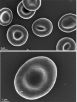
\includegraphics[width=0.3\textwidth]{../Figuras/SEM_erythrocyte.pdf}\label{subfig:SEM}}}\hspace{0.5cm}
	\sidesubfloat[Second image]{\hspace{-0.5cm}{	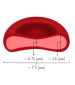
\includegraphics[width=0.37\textwidth]{../Figuras/erythrocyte.pdf}\label{subfig:ery}}}
	\caption{Estructura de un eritrocito sano. \textbf{a)} Micrografías SEM de eritrocitos de pacientes sanos. La micrografía superior muestra eritrocitos de forma bicóncava normal con interacción limitada, mientras que la inferior muestra un eritrocito sano con una membrana ligeramente granular; imágenes extraídas y adaptadas de \cite{alummoottilScanningElectronAtomic2023}. \textbf{b)} Diagrama de un corte longitudinal de un eritrocito que muestra las dimensiones de la célula. }
	\label{fig:erythrocytes}
\end{figure}


\begin{figure}[t]
	\centering
	\sidesubfloat[First image]{\hspace{-0.5cm}{
		
\includegraphics[width=0.32\textwidth]{../Figuras/erythrocyte_health.pdf}\label{subfig:ery_health}}}\hspace{0.9cm}
	\sidesubfloat[Second image]{\hspace{-0.3cm}{	
\includegraphics[width=0.247\textwidth]{../Figuras/spherocytosis.pdf}\label{subfig:spherocyte}}}
	
	\vspace{0.3cm}
	
	\sidesubfloat[Third image]{\hspace{-0.5cm}{	
\includegraphics[width=0.29\textwidth]{../Figuras/microcyte.pdf}\label{subfig:microcyte}}}	\sidesubfloat[Fourth image]{\hspace{-0.3cm}{	
\includegraphics[width=0.32\textwidth]{../Figuras/macrocyte.pdf}\label{subfig:macrocyte}}}
	
	
	\caption{Morfologías de eritrocitos sanos y patológicos. \textbf{a)} Eritrocito sano con forma bicóncava y radio menor a 3.75~$\mu$m. \textbf{b)} Esferocito: eritrocito con el mismo volumen que un eritrocito sano pero con radio menor. \textbf{c)} Microcito: eritrocito de menor tamaño que uno sano. Conserva la forma bicóncava. \textbf{d)} Macrocito: eritrocito de mayor tamaño que uno sano. Conserva la forma bicóncava.  }
	\label{fig:erythrocytes_diseases}
\end{figure}

La geometría, el tamaño y el índice de refracción de los eritrocitos son susceptibles a alteraciones con relevancia clínica, influyendo tanto en su funcionalidad fisiológica como en su comportamiento óptico \cite{ergulComputationalStudyScattering2010a}. Su clasificación suele basarse en parámetros hematológicos, como la CHCM, que cuantifica la concentración promedio de hemoglobina en el eritrocito \cite{bosschaartLiteratureReviewNovel2014a}, y en su morfología, incluyendo el radio y el volumen celular. Ante diversas patologías, el eritrocito puede sufrir alteraciones como las mostradas en la Fig.~\ref{fig:erythrocytes_diseases}. La Fig.~\ref{subfig:ery_health} presenta un eritrocito sano, con las dimensiones indicadas previamente en la Fig.~\ref{subfig:ery}. Los eritrocitos sanos presentan valores de CHCM entre 30 y 32 g/dL \cite{saxenaClinicalEvaluationDifferent2018}. En contraste, la Fig.~\ref{subfig:spherocyte} muestra un esferocito, caracterizado por tener un volumen igual o similar al de un eritrocito sano, pero con una superficie celular reducida debido a defectos en las proteínas responsables de mantener la unión adecuada entre el citoesqueleto y la bicapa lipídica \cite{donatoEsferocitosisHereditariaRevision2015}. Como consecuencia, la célula adquiere una forma esférica con una menor relación superficie–volumen y posee valores de CHCM mayores a 32 g/dL \cite{saxenaClinicalEvaluationDifferent2018}. Esta alteración incrementa la tensión de membrana y la vuelve más frágil e incapaz de adaptarse a variaciones fisiológicas \cite{donatoEsferocitosisHereditariaRevision2015}. La Fig.~\ref{subfig:microcyte} muestra un microcito, definido como un eritrocito de tamaño reducido (diámetro menor que $ 7~\mu$m y, a menudo, CHCM menor que $ 30~\text{g/dL}$) \cite{saxenaClinicalEvaluationDifferent2018}. Suelen asociarse con hipocromía y con trastornos que afectan el metabolismo del hierro o la síntesis de hemoglobina \cite{ergulComputationalStudyScattering2010a}. Por otro lado, en la Fig.~\ref{subfig:macrocyte} se observa un macrocito, identificado por un diámetro mayor a $ 8.5~\mu\text{m}$ y CHCM de aproximadamente $34~\text{g/dL}$ \cite{saxenaClinicalEvaluationDifferent2018}. Aunque su forma puede seguir siendo bicóncava, su tamaño aumentado suele relacionarse con alcoholismo crónico, enfermedades hepáticas, deficiencias vitamínicas, mieloma o leucemia \cite{ergulComputationalStudyScattering2010a}. 
  
  Las modificaciones en la geometría (radio celular y volumen) y la composición interna (CHCM) que caracterizan a estas patologías, alteran el índice de refracción y las propiedades de esparcimiento óptico de los eritrocitos \cite{bosschaartLiteratureReviewNovel2014a}. Por lo tanto, en el estudio de las propiedades ópticas de la sangre en estas condiciones se requiere la implementación de modelos que contemplen con precisión la morfología y la composición interna de los glóbulos rojos patológicos, estableciendo un contraste con las propiedades de los eritrocitos sanos.


